\documentclass[a4paper,11pt]{article}

\usepackage{clrscode}

\usepackage{geometry}
\geometry{
 a4paper,
 left=30mm,
 top=30mm,
}
\usepackage[utf8]{inputenc}

\usepackage{graphicx}
\usepackage[english]{babel}
\usepackage{color}
\usepackage[dvipsnames]{xcolor}
\usepackage[colorlinks=true,urlcolor=blue,citecolor=black]{hyperref}
\usepackage{url}
%\urlstyle{same}
%\urlstyle{rm}
\urlstyle{sf}
%\urlstyle{tt}
\usepackage[font=footnotesize,labelfont=bf]{caption}
\usepackage[labelfont=it,textfont={it},singlelinecheck=on,justification=centering]{caption}
%full name for appendix
\usepackage[title]{appendix}
\usepackage{float}
\setlength{\parindent}{2em}
\usepackage{parskip}
%for code
\usepackage{listings}
%for math
\usepackage{amsmath}
\usepackage{breqn}
\usepackage{pdfpages}
\linespread{1.1}
\setlength{\emergencystretch}{3em}

\usepackage{ifxetex,ifluatex}
\usepackage{etoolbox}
\usepackage{tikz}

\usepackage{framed}

%water mark
\usepackage{eso-pic}

\newcommand{\watermark}[3]{\AddToShipoutPictureBG{
	\parbox[b][\paperheight]{\paperwidth}{
		\vfill%
		\centering%
	\tikz[remember picture, overlay]%
	  \node [rotate = #1, scale = #2] at (current page.center)%
	      {\textcolor{gray!80!cyan!30}{#3}};
	  \vfill}}}
\usepackage{blindtext}
%water mark end


% conditional for xetex or luatex
\newif\ifxetexorluatex
\ifxetex
  \xetexorluatextrue
\else
  \ifluatex
    \xetexorluatextrue
  \else
    \xetexorluatexfalse
  \fi
\fi
%
\ifxetexorluatex%
  \usepackage{fontspec}
  \usepackage{libertine} % or use \setmainfont to choose any font on your system
  \newfontfamily\quotefont[Ligatures=TeX]{Linux Libertine O} % selects Libertine as the quote font
\else
  \usepackage[utf8]{inputenc}
  \usepackage[T1]{fontenc}
  \usepackage{libertine} % or any other font package
  \newcommand*\quotefont{\fontfamily{LinuxLibertineT-LF}} % selects Libertine as the quote font
\fi

\newcommand*\quotesize{60} % if quote size changes, need a way to make shifts relative
% Make commands for the quotes
\newcommand*{\openquote}
   {\tikz[remember picture,overlay,xshift=-4ex,yshift=-2.5ex]
   \node (OQ) {\quotefont\fontsize{\quotesize}{\quotesize}\selectfont``};\kern0pt}

\newcommand*{\closequote}[1]
  {\tikz[remember picture,overlay,xshift=4ex,yshift={#1}]
   \node (CQ) {\quotefont\fontsize{\quotesize}{\quotesize}\selectfont''};}

% select a colour for the shading
\definecolor{mygray}{gray}{0.95}
\colorlet{shadecolor}{mygray}

\newcommand*\shadedauthorformat{\emph} % define format for the author argument

% Now a command to allow left, right and centre alignment of the author
\newcommand*\authoralign[1]{%
  \if#1l
    \def\authorfill{}\def\quotefill{\hfill}
  \else
    \if#1r
      \def\authorfill{\hfill}\def\quotefill{}
    \else
      \if#1c
        \gdef\authorfill{\hfill}\def\quotefill{\hfill}
      \else\typeout{Invalid option}
      \fi
    \fi
  \fi}
% wrap everything in its own environment which takes one argument (author) and one optional argument
% specifying the alignment [l, r or c]
%
\newenvironment{shadequote}[2][l]%
{\authoralign{#1}
\ifblank{#2}
   {\def\shadequoteauthor{}\def\yshift{-2ex}\def\quotefill{\hfill}}
   {\def\shadequoteauthor{\par\authorfill\shadedauthorformat{#2}}\def\yshift{2ex}}
\begin{snugshade}\begin{quote}\openquote}
{\shadequoteauthor\quotefill\closequote{\yshift}\end{quote}\end{snugshade}}


\usepackage{listings}
\lstdefinestyle{myListStyle}{
  numbers=left,
  stepnumber=1,
  numbersep=10pt,
  tabsize=2,
  showspaces=false,
  showstringspaces=false
}

\usepackage[dvipsnames]{xcolor}
\usepackage{listings}

\newcommand\YAMLcolonstyle{\color{darkgray}\mdseries}
\newcommand\YAMLkeystyle{\color{black}\bfseries}
\newcommand\YAMLvaluestyle{\color{gray}\mdseries}

\makeatletter

% here is a macro expanding to the name of the language
% (handy if you decide to change it further down the road)
\newcommand\language@yaml{yaml}

\expandafter\expandafter\expandafter\lstdefinelanguage
\expandafter{\language@yaml}
{
  keywords={true,false,null,y,n},
  keywordstyle=\color{darkgray}\bfseries,
  basicstyle=\YAMLkeystyle,                                 % assuming a key comes first
  sensitive=false,
  comment=[l]{\#},
  morecomment=[s]{/*}{*/},
  commentstyle=\color{black}\ttfamily,
  stringstyle=\YAMLvaluestyle\ttfamily,
  moredelim=[l][\color{orange}]{\&},
  moredelim=[l][\color{magenta}]{*},
  moredelim=**[il][\YAMLcolonstyle{:}\YAMLvaluestyle]{:},   % switch to value style at :
  morestring=[b]',
  morestring=[b]",
  literate =    {---}{{\ProcessThreeDashes}}3
                {>}{{\textcolor{red}\textgreater}}1
                {|}{{\textcolor{red}\textbar}}1
                {\ -\ }{{\mdseries\ -\ }}3,
}

% switch to key style at EOL
\lst@AddToHook{EveryLine}{\ifx\lst@language\language@yaml\YAMLkeystyle\fi}
\makeatother

\newcommand\ProcessThreeDashes{\llap{\color{cyan}\mdseries-{-}-}}



%opening
\title{\LARGE The Qitmeer White Paper:\\
	\Large The guardian of trust.}
\author{
	Qitmeer team\\
		\small\href{mailto:paper@qitmeer.io}
			{\nolinkurl{paper@qitmeer.io}}
	}
\date{\today\\\small Version 0.4.1}
\begin{document}

%% Cover end
\clearpage
\pagestyle{plain}

\maketitle

%\watermark{60}{10}{qitmeer.io}

\begin{abstract}
Bitcoin\cite{bitcoin} was born with revolution which opened a new horizon of currency issuance that becomes open and fair by a cryptography-based decentralized payment network. The underlying ledger mechanism of Bitcoin (blockchain), is capable of playing a significant role in the financial system due to its tamper resistance. The Blockchain technology will reshape Interest-free finance, as a significant alternative system of global financial system.

With the arrival of 10-years birth of bitcoin, the blockchain infrastructure is facing various challenges from technical perspective. Moreover, Qitmeer considers openness, fairness, fault tolerance, scalability as the core metrics to assess a promising blockchain paradigm, and a blockchain system achieved a desirable balance among these metrics is regarded as Classical Blockchain Setting.

Qitmeer Consensus adopts the SPECTRE\cite{SPECTRE}  as its fundamental protocol. SPECTRE is a fast confirmation and high throughput BlockDAG protocol, which guarantees high performance in a payment network. Additionally, Qitmeer incorporates  another high throughput BlockDAG protocol   GhostDAG\cite{GhostDAG}, which is highlighted on unprecedentedly supporting transactions linearly ordering, to circumvent SPECTRE’s weak liveness and provide ordering service for the fair scheme of the reward system. The Qitmeer Consensus is in line with Classical Blockchain Setting which could join and leave the network freely by Proof-of-Work, with the collaboration model of DAG ledger guarantees that miners gain rewards corresponding to their contribution respectively, the  50\% fault tolerance as secure as bitcoin, robust scalability that is subjected to physical network limit. The mining algorithm is also a vital source of fairness other than consensus algorithm per se. Cuckoo Ring is a graph theory based proof-of-work mining algorithm and is practically ASIC resistant due to memory-hard calculation. 

According to Shariah requirements, Qitmeer designs a UTXO-based unique token issuance scheme, which has effectively solved two main challenges: Intrinsic Value and Assets Authentication. Issuing a certain amount of assets must consume a certain amount of the native currency. Moreover, the entity must be warranted a license to issue assets. 

Qitmeer devises a set of specifications and protocols to be adopted in the Global Islamic economy ecosystem, such as wallets and miners. As for interoperability, Qitmeer recognises the utilizing of cross-chain protocols to integrate various cryptocurrencies and offer reliable off- chain smart contract services.

\end{abstract}

\section{Introduction}

\subsection{Background}
Trust is the cornerstone of financial system, while in traditional approach, multiple unacquainted parties require a trustworthy third party to guarantee the security of transactions. However, the third party is centralized and subject to single point failure, unlikely to guarantee its honesty.

Bitcoin is an open P2P network, meaning that there does not exist a centralized server, each node can join or leave the network freely. The calculation-heavy but validation-easy Proof-of-Work consensus is designed to ensure nodes gain rewards relevant to their contribution to the network’s running security, which is supposed to be fair. Bitcoin has a hash-list-like ledger to guarantee tamper resistance, this disruption has been driving tons of researches on its working mechanism. The concept of ’BlockChain’ is introduced to represent this mechanism and commonly accepted. Owing to trustlessness and tamper resistance, an increasing number of applications of blockchain occur in the financial system which acts as the new driving force to re-shape the financial system.

With the innovation of Bitcoin ten years ago, the blockchain infrastructure is facing various challenges from technical perspective and has been deviating from its essence philosophy. Bitcoin is no longer decentralized, the top five mining pool has controlled majority hash power and would be easy to carry on an attack if there is any reason. Miners have to join mining pools since the opportunity cost is much higher than their contribution. In other word, Bitcoin is not fair any more, because Bitcoin does not scale, seven transactions per second throughput, one hour confirmation time, high cost of the transaction fee, far from promising as a global payment network.

Bitcoin needs to be reformed to reflect its essence philosophy. There are Countless solutions claim themselves to have been solved all these challenges. However, few achieved indeed, just trading off one metric with another, like sacrifice decentralization, which is the core source of security for scalability. So, what is the essence philosophy of bitcoin? Qitmeer has defined it as Classical Blockchain Setting, which has deeply innovated design philosophy of Qitmeer network.

\subsection{Classical Blockchain Setting}
There are many blockchain evolves and each has its own definition of blockchain technology. However, Qitmeer network acknowledged  bitcoin’s objectives, Qitmeer holds the view that the following four metrics as Classical Blockchain Setting.

\subsubsection{Openness}
Openness is an essential feature to distinguish permissioned and permissionless blockchain, which means every node should join and leave the network freely.


\subsubsection*{Predefined special roles}
An open network allows different roles, in the bitcoin network, nodes could choose to be an SPV(Simplified Payment Verfication( node, full node or miner with freedom, so from the protocol’s aspect, bitcoin is open. Whereas, in Delegated Proof-of-Work, the block producers are voted off the chain with predefined  configurations,which demonstrates limited openness in the network.

\subsubsection*{Practically closed}
Bitcoin is defined as open source according to the protocol, it is actually closed in practice. Miners have to join mining pools to minimize the risk of opportunity costs, at the expense to lose their free will. The situation is getting deteriorating in a speedy manner as described above. 


\subsubsection{Fairness}
Fairness means that the rewards should be consistent with the contribution in the network which is Incentive-Compatibility.

\subsubsection*{Opportunity Cost}
The expectation of rewards between solo mining and pool mining is equal in terms of probability. The point is, their opportunity cost is considerably high - either mine a block to get a dramatically high reward or wait a long time without any return. Therefore, miners have to turn to the mining pool to have a stable incentive.

\subsubsection*{Cost Efficiency}
Cost Efficiency is referring to mining cost. Mining cost mainly includes the electricity price and mining efficiency, and the latter is much more critical due to ASIC. ASIC is customized to direct a specific mining algorithm, so the mining efficiency per unit of cost is much higher than gener- alized computers. For instance, the hash rate per dollar for AntMiner S9 is about 20000 times greater than for GTX570; it is nearly impossible for a personal computer to win the hash rate competition.

\subsubsection{Secure}
The security is how robust the network is to sustain the attack, mainly referring to overrun a confirmed transaction.

\subsubsection*{Decentralization}
Decentralization is the most significant feature of bitcoin to be compared with traditional payment network. Decentralization could avoid single point failure on account of the fact that it is almost impossible to collude with the majority of all nodes in a fully decentralized network.
\subsubsection*{Fault Tolerance}
Fault Tolerance refers that the network should be resilient to a certain proportion of malfunctioning resources, and fault tolerance is the upper bound of the percentage. In a decentralized network, 50\% fault tolerance is the desirable case according to the majority law.

\subsubsection{Scalable}
A network that can offer relatively stable services with its scale increasing is considered scalable. Blockchain network includes the following services:
\subsubsection*{Throughput}
The throughput is the number of transactions per second (TPS) and its performance is of essential importance when network is scaling, while up to present, Bitcoin’s throughput is upper bound to 7 TPS despite of  how many nodes are available there in the network, which limits itself to act as the global payment network.
\subsubsection*{Confirmation}
The confirmation is the time that the recipient to wait until the transaction is unlikely to be reversed, which should not be increased with networking scaling. In bitcoin network, the confirmation time is six blocks or one hour.  Confirmation affects user experience significantly, especially in a payment network, users won’t stand to wait too long to accept their transactions.
\subsubsection*{Cost}
The main component of cost is transaction fee which should be maintained in a  reasonable range, since it would make payment impractical if too high, or it would be subject to sybil-attack if it is too low. With the mining difficulty increasing, Bitcoin transaction fee is getting higher and higher, and it won’t be suitable to serve as a global payment network as it aims to be, up to present, the average price of bitcoin is roughly 2\$. 

\subsection{Specification}
The Qitmeer network specification is designed to follow Classical Blockchain Setting. The four metrics have some intrinsic contradiction among each other, Qitmeer cannot achieve best in each simultaneously, but find an optimized balance, i.e., seek for high scalability based on an open, fair and secure network.
\subsubsection{Openess}
Proof-of-Work is the openest way to join a blockchain network due to the only resource required is electricity, which is physical and owned by each of the nodes.  
\subsubsection*{Proof of Work}
Proof-of-Work is the openest way to join a blockchain network due to the only resource required is electricity, which is physical and owned by each of the nodes.  

Proof-of-Work is the openest way to join a blockchain network due to the only resource required is electricity, which is physical and owned by each of the nodes.  

\subsubsection*{No Predefined Nodes}
Predefined Nodes refer to special nodes defined in the protocol. Note: though there are mining pools in bitcoin,  they are unexpected in bitcoin protocol. Thus,  bitcoin still has no predefined nodes, so does Qitmeer because it is in line with bitcoin’s paradigm.
\subsubsection{Fairness}
BlockDAG is fair due to its adoption of a collaboration model instead of competition model of blockchain.
\subsubsection*{Mining Pool Resistance}
Mining pools centralization is the consequence of high opportunity cost, which is the conse- quence of the competition model. Qitmeer’s BlockDAG-based protocol SPECTRE is a collabo- ration model, the opportunity cost of solo mining is equal to that of pool mining. As a miner either individually or collectively, it is not compulsory to join a mining pool, which would lead to the risk of centralization.
\subsubsection*{Anti-ASIC Mining Algorithm}
Cuckoo Cycle is a graph-theoretic proof-of-work algorithm which prevails for ASIC resistance. Qitmeer adopts this algorithm to guarantee that no one has too much mining efficiency advantage.
\subsubsection{Security}
Security is the top consideration in the Qitmeer network. Qitmeer has achieved fully decentralized and 50\% fault tolerant. Thus, there is no compromise to trade-off security with other metrics.
\subsubsection*{Fully Decentralization}
All the nodes in the Qitmeer’s network are peer nodes and are entitled to participate in consensus.
\subsubsection*{50\% Faulty Tolerance}
The malicious adversary has to possess 50\% hash power to control the network. Either in SPECTRE or GhostDAG, the fault tolerance is irrelevant with the throughput, whereas the security is inversely proportional to throughput in bitcoin.

\subsubsection{Scalability}
There are features of Qitmeer network such as high scalability, fast confirmation, high throughput, and low transaction fees, that could ensure Qitmeer will be running stably in a considerable long time.

\subsubsection*{Fast Confirmation}
The Qitmeer adopts the SPECTRE as consensus algorithm which is a speedy confirmation BlockDAG protocol. 
\subsubsection*{High Throughput}
SPECTRE is a BlockDAG protocol, and the throughput could employ full potential performance subject to the network’s physical metrics, such as network bandwidth or propagation delay.
\subsubsection*{Low Cost}
Technically, the cost is not scaling since the transaction fee is increasing slightly with the network growing. However, the average cost will keep relatively insignificant and reasonable for a long period.  

\section{Qitmeer Token Design}
The existing blockchain networks have not taken into consideration the  Shariah compliance and ethical concern entirely, from its whole ecosystem when they initiate their design. However, Qitmeer has taken Shariah Compliance into consideration rooted from its underlying philosophy, and penetrated through the whole technical architecture , until the applications in the ecosystem, in which it has been designed an effective approach, namely OP_TOKEN.

\subsection{Background}
\subsubsection{Problem definition}

Blockchains are ought to consider two main points to be considered as Shariah compliance in the Blockchain industry:

\subsubsection*{Intrinsic Value}
Assets must have underlying value and cannot be created out of thin air. On existing token issuance platforms like Ethereum\cite{Ethereum}, individuals can issue a token of arbitrary amount without any foundation.
 

\subsubsection*{Assets Authentication}
The blockchain should not allow any issuance of illegitimate assets and unethical business. Existing blockchains are too unrestricted in the event of assets authentication.

\subsubsection{Related works}

The $\texttt{OP\_TOKEN}$ is inspired by Color coin idea, which represents and manages real-world assets on top of the Bitcoin by using $\texttt{OP\_RETURN}$, and the OP\_GROUP, a referenced implementation of issuing assets designed by Andrew Stone.

The OP\_TOKEN fit various practical scenarios with unique features like asset compliable and value relevent. There are some related concepts in the details below:

\subsubsection*{UTXO}

The Unspent Transaction Outputs (UTXO) are used whether the transaction is valid. there are no accounts required in Qitmeer network. What users have in the network and spend are a bunch of unspent transaction output. This could come up with the balance by summing up UTXO.

\begin{figure}[hbt]
	\centerline{%
	   \resizebox{0.8\textwidth}{!}{\includegraphics{figures/UTXO}}%
	}
\caption{utxo model}
\end{figure}

The first transaction tx1 has three outputs with the first spent, so  tx1 has 2+3=5 coins balance.

The second transaction tx2 spends the 2 UTXOs of tx1 and pays to 3 addresses and creates three new UTXOs.

Note: now the old UTXOs (of tx1) are no longer UTXO so cannot be spent later.

\subsubsection*{Script system}

The mechanism behind how users spend their UTXOs is to execute a particular script. The output stores half of the script and it has to present the other half and combine both in order to verify if the money is spent. The former half is called locking script, like a locked treasure box, and the latter is unlocking script, like the only key to the box.

For example, a typical instance of  Pay-2-Public-Key-Hash(P2PKH)\cite{P2PKH} Locking Script in UTXO:

\begin{lstlisting}
OP_DUP OP_HASH160 <PUBLIC_KEY> OP_EQUALVERIFY OP_CHECKSIG
\end{lstlisting}

Unlocking Script in a newly created transaction:

<Signature><PublicKey>

Combine unlocking script with locking script:

<Signature><PublicKey> OP\_DUP OP\_HASH160 <PUBLIC\_KEY> OP\_EQUALVERIFY OP\_CHECKSIG

This whole script consists two steps
1. <PublicKey>  OP\_HASH160 <PUBLIC\_KEY> OP\_EQUALVERIFY
	To verify if the public key in the unlocking script matches that in the locking script.
2.  <Signature><PublicKey> OP\_CHECKSIG
	To check if the signature is valid.


\subsubsection*{Colored coins and Tether}

Colored Coins\cite{ColoredCoins} is a method that represent assets on blockchain, it can leverage the tamper-proof capability of blockchain. However, It uses transaction script operation $\texttt{OP\_RETURN}$ to interrupt script execution early. Therefore, it can add information to the assets after OP\_RETURN without violating the script validation. 

Locking Script:
\begin{lstlisting}
OP_RETURN <DATA>
\end{lstlisting}

Moreover, the stable coin Tether\cite{Tether} (USDT) also uses OP\_RETURN based OMNI Layer protocol to define the asset on the bitcoin.

Here are a typical USDT transaction and details of its protocol design


\lstset{basicstyle=\tiny,style=myListStyle}
\begin{lstlisting}
OP_RETURN 6f6d6e69000000000000001f00000015c9054900
\end{lstlisting}


\begin{figure}[hbt]
	\centerline{%
	   \resizebox{0.8\textwidth}{!}{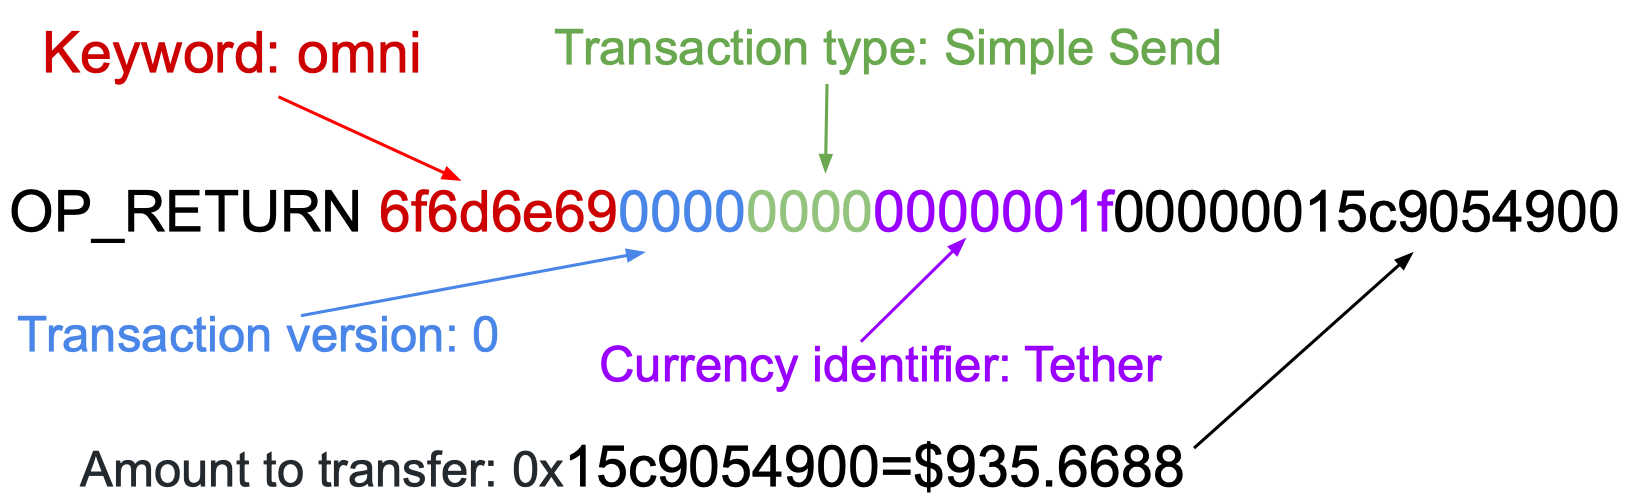
\includegraphics{figures/USDT}}%
	}
\caption{USDT}
\end{figure}


%[ref][https://www.blockchain.com/btc/tx/efc50d9e1f23e687e304cfca4ef2c5412b67d5737888ff80a0cbb6853cd865c]



\subsubsection*{OP\_GROUP}
The OP\_RETURN  scheme is more suitable to apply on mature blockchain, since it does not change the underlying blockchain protocol and will not risk forking. However, the weakness is that miners cannot verify its protocol, so there would be some security risks.

OP\_GROUP\cite{OP_GROUP}  is an improvement proposal of assets issuance on Bitcoin Cash (BCH)\cite{BCH} from Bitcoin Unlimited (BU). Thus, OP\_GROUP  supports transfer, destroy and insurance of Token. Since OP\_GROUP is an extension to the BCH script system,  it is part of the BCH protocol. Thus miners can do the verification, which is more reliable.

The basic “colored” pay 2 public key hash script would be like:

\lstset{basicstyle=\tiny,style=myListStyle}
\begin{lstlisting}[numbers=none]
OP_DATA(group address)
OP_GROUP
OP_DROP
OP_DUP
OP_HASH160
OP_DATA(pubkeyhash)
OP_EQUALVERIFY
OP_CHECKSIG
\end{lstlisting}

The main difference is simple, just adding a group address to distinguish different groups, and other operations, such as create and destroy assets, are similar.

% [ref]https://medium.com/@g.andrew.stone/bitcoin-scripting-applications-representative-tokens-ece42de81285

\subsection{OP\_TOKEN Design}

\subsubsection{Overview}

There is a unique token named LICENSE in OP\_TOKEN. The relevant regulatory bodies, shariah-governance entities, industry practitioners with public credibility within the ecosystem are invited to receive the licences to oversight the compliances issues that might occur along the course of mainstream adoption of the protocol. Any entity planning to issue a token needs to be warranted with a license. Peers can transfer licenses as they are also tokens in nature. However, the originator must be extra careful in event of transferring in order to avoid non-compliance risk due to the records is public and immutable.  
 

\subsubsection{Issuance of License}

Licenses are all generated in the genesis block and distributed to C preserved committee members. One smallest unit (SAND) can represent a license, one block has M coins, one coin= N SAND, so we have M*N license in total, which is sufficient for asset issuance.


\begin{lstlisting}[language=yaml, numbers=none,basicstyle=\footnotesize]
# C = 100, M = 10, N = 10^8 (M*N = 10 billion),
# all examples are based on this setting
# Ex1: Distribute licenses to the commitee,
# M*N/C = 100 million for each member.
---
INPUTS:
	INPUT:
		PREVIOUS_OUTPUT: # (COINBASE of GENESIS)
			S: "DUP HASH160 [GEN] EQUALVERIFY CHECKSIG"
			V: 10000000000
		S: "[SIG] [GEN_PK]"
OUTPUTS:
	OUTPUT:
		S: "[LIC] TOKEN DROP DUP HASH160 [COMM1] EQUALVERIFY CHECKSIG"
		V: 100000000
	# ... ... (COMMITTEE MEMBER 2~99)
	OUTPUT:
		S: "[LIC] TOKEN DROP DUP HASH160 [COMM100] EQUALVERIFY CHECKSIG"
		V:100000000
	OUTPUT:
		S: "RETURN [DATA]"
		V: 0
\end{lstlisting}



\subsubsection{Warrant a license}

The relevant entities must be warranted a license to issue assets. The entity can request a license from any committee member (C.M.). Once the license is granted and approved. These entities will receive a particular token transfer from the C.M. and the Token is the licensed.

\lstset{basicstyle=\tiny,style=myListStyle}
\begin{lstlisting}[language=yaml, numbers=none,basicstyle=\footnotesize]
# Ex2: C.M. warrant a license to the issuer (ISS),
# note the license change will go back to the C.M.
---
INPUTS:
	- INPUT:
			PREVIOUS_OUTPUT:
				S: "[LIC] TOKEN DROP DUP HASH160 [COMM] EQUALVERIFY CHECKSIG"
				V: 100000000
			S: "[SIG] [COMM_PK]"
OUTPUTS:
	- OUTPUT:
			S: "[LIC] TOKEN DROP DUP HASH160 [ISS] EQUALVERIFY CHECKSIG"
			V: 1
	- OUTPUT: # License change
			S: "[LIC] TOKEN DROP DUP HASH160 [COMM] EQUALVERIFY CHECKSIG"
			V: 99999999
	- OUTPUT:
			S: "RETURN [DATA]"
			V: 0
\end{lstlisting}

\subsubsection{Issuance of assets}
Once the license is warranted, entities can issue assets; however, they cannot set the token amount arbitrarily. Instead, to issue a certain amount of assets requires converting the same amount of SANDs. The Qitmeer network calls this process as "token mint". Just like the case in reality, to mint a gold coin requires the same weight of gold sands, tokens need the same amount of SANDs.

The first advantage of issuance system is to guarantee tokens’ elementary intrinsic value; thus, it would significantly mitigate the price fluctuation. Another advantage is that tokens and native currency are no longer isolated islands of value; which are running in the same ecosystem and would improve the liquidity and make the whole network stable.

\lstset{basicstyle=\tiny,style=myListStyle}
\begin{lstlisting}[language=yaml, numbers=none,basicstyle=\footnotesize]
# Ex3: Convert 100000000 native SANDs, i.e. 1 Coin,
# to 100000000 sands of the new token,
# note the license will go back to the issuer for future issurance.
INPUTS:
	- INPUT:
			PREVIOUS_OUTPUT: #(1 LICENSE)
				S: "[LIC] TOKEN DROP DUP HASH160 [ISS] EQUALVERIFY CHECKSIG"
				V: 1
			S: "[SIG] [LIC_PK]"
	- INPUT:
			PREVIOUS_OUTPUT: #(1 Qitmeer Coin)
				S "DUP HASH160 [COIN] EQUALVERIFY CHECKSIG"
				V: 100000000
			S: "[SIG] [COIN_PK]"
OUTPUTS:
	- OUTPUT: # License returns to the issuer
			S: "[LIC] TOKEN DROP DUP HASH160 [ISS] EQUALVERIFY CHECKSIG"
			V: 1
	- OUTPUT:
			S: "[TOK] TOKEN DROP DUP HASH160 [PK] EQUALVERIFY CHECKSIG"
			V: 100000000
	- OUTPUT:
			S: "RETURN [DATA]"
			V: 0
\end{lstlisting}

\subsubsection{Transfer of the Assets}

The entities can transfer assets to each other. Moreover, the entity could transfer multiple assets within one transaction. The transaction needs to ensure the input sum of each asset equals the output sum of each asset.

\lstset{basicstyle=\tiny,style=myListStyle}
\begin{lstlisting}[language=yaml, numbers=none,basicstyle=\footnotesize]
# Ex4: Alice exchanges her 100 RMB token with Bob's 20 USD token.
INPUTS:
	- INPUT:
			PREVIOUS_OUTPUT:
				S: "[RMB] TOKEN DROP DUP HASH160 [A_PKH] EQUALVERIFY CHECKSIG"
				V: 100
			S: "[A_SIG] 0X83 [A_PK]"
	- INPUT:
			PREVIOUS_OUTPUT:
				S: "[USD] TOKEN DROP DUP HASH160 [B_PKH] EQUALVERIFY CHECKSIG"
				V: 20
			S: "[B_SIG] 0X83 [B_PK]"
OUTPUTS:
	- OUTPUT:
			S: "[USD] TOKEN DROP DUP HASH160 [A_PKH] CHECKSIG"
			V: 20
	- OUTPUT:
			S: "[RMB] TOKEN DROP DUP HASH160 [B_PKH] CHECKIG"
			V: 100
\end{lstlisting}


\subsubsection{Melt Token}

Melt is the reversed process of mint, i.e., conversion from tokens to native currency. The total amount of sand is constant, either in the form of Native Sand or Token Sand. However, it is allowed to transform a token and convert native currency. Issuers can melt their coins to reduce liquidity in order to keep the price stable, which is practical to implement stable coins. Melt guarantees the tokens fundamental value, just like the minimum value of a gold coin is the same weight of gold.   


Melt guarantees the tokens fundamental value, just like the minimum value of a gold coin is the same weight of gold.

\lstset{basicstyle=\tiny,style=myListStyle}
\begin{lstlisting}[language=yaml, numbers=none,basicstyle=\footnotesize]
# Ex5: Melt 100 token sands into 100 native sands
INPUTS:
	- INPUT:
			PREVIOUS_OUTPUT:
				S: "[TOK] TOKEN DROP DUP HASH160 [ISS] EQUALVERIFY CHECKSIG"
				V: 100
			S: "[SIG] [ISS_PK]"
OUTPUTS:
	- OUTPUT:
			S: "DUP HASH160 [COIN] EQUALVERIFY CHECKSIG"
			V: 100
	- OUTPUT:
			S: "RETURN [DATA]"
		V: 0
\end{lstlisting}


\section{Consensus Protocol}


\subsection{From BlockChain To BlockDAG}
Bitcoin does not scale due to protocol restrain. By Nakamoto Consensus, i.e., longest-chain rule, 1 MB block size and 10 minutes block rate confine bitcoin to reach only 7 TPS theoretical throughput regardless of the bandwidth and propagation delay.

The most intuitive way to increase scalability is to shorten block time or enlarge block size. The reason why Satoshi did not adopt is because that will bring forks, as well as distracting the hash power from the main chain, thus causing security vulnerability.

GHOST protocol introduces heaviest-tree consensus to keep forks without sacrificing security. Note that here BlockChain has transformed into a BlockTree. Since the largest subtree has concentrated the majority hash power, the security is as high as bitcoin. The main chain is the path, i.e. a blockchain from the genesis to leaf, with the highest number of descendants, other blocks are off-chain blocks. Only main chain blocks contribute throughput, off-chain blocks help strengthen the security. 

BlockTree has dramatically increased throughput because of the higher Block Rate or Size. However, there is still a waste of the transactions of off-chain blocks, which should contribute to the throughput as well. Inclusive protocol proposes a new data structure of ledger, where every block confirms every unconfirmed block. This improvement upgrades a BlockTree to a BlockDAG.

Through the development history from BlockChain to BlockDAG, it may indicate  that BlockChain is a particular case of BlockDAG in the event of low throughput, which means both are the same in essence. As a result,  it is the scaling approach whose paradigm is the closest to the bitcoin network. BlockDAG is robust since it inherits all the long-time-proved stable features of bitcoin,  as well as it could scale infinitely in terms of protocol, unless it is limited physically, such as, bandwidth. A robust public chain is the optimal basis for incorporating further scaling solutions, such as sharding and state-channels, thus BlockDAG is the preferred scaling solution of Qitmeer.


\begin{figure}[hbt]
	\centerline{%
	   \resizebox{0.8\textwidth}{!}{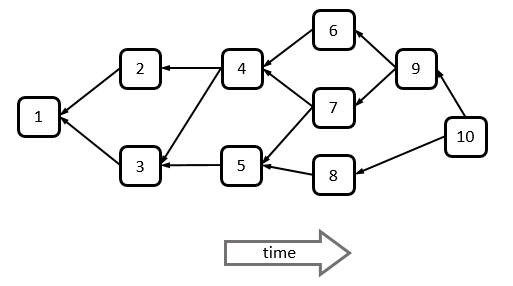
\includegraphics{figures/DAG.png}}%
	}
\caption{DAG}
\end{figure}

\subsection{Consensus}

Qitmeer adopts a hybrid consensus that combines SPECTRE and GHOSTDAG in order to achieve fast confirmation and high throughput.

\subsubsection{SPECTRE}
SPECTRE\cite{SPECTRE} is a BlockDAG based protocol that achieves fast confirmation and high throughput with 50\% attack resilience. SPECTRE guarantees safety, which means the transaction is unlikely to be reversed once it is accepted. However, the SPECTRE guarantees fast confirmations for honest users rather than all users which is weak liveness.

There is a trade-off between liveness and fast confirmation, whereby SPECTRE prioritizes the latter due to weak liveness only affects malicious users, that enables SPECTRE to be a suitable protocol for payment model. In the event malicious users launch double spending attack, their transactions are likely to be delayed indefinitely.

SPECTRE is a stateless transaction model, whereby there is no need to gain a total ordering over all the blocks. Only when two blocks conflicting that a pairwise ordering is needed. SPECTRE employs a voting algorithm to decide which block wins when there is a conflict between two blocks. Suppose block x has a conflicting transaction with another transaction in block y, and also suppose that block z is voting on them with the following rules:

SPECTRE employs a voting algorithm to decide which block wins when two blocks
conflict. Suppose block $x$ has a conflicting transaction with another
transaction in block $y$, and also suppose that block $z$ is voting on them with
the following rules:

\begin{enumerate}
	\item If $z$ is in $x$'s future but not in $y$'s future, $z$ votes for
		$x$ in favor of $y$, denoted as $x \prec y$, and vice versa.
	\item If both $x$ and $y$ are in the past of $z$, then $z$ follows the majority votes in its past.
	\item If neither $x$ nor $y$ is in the past of $z$, then $z$ follows the majority votes in its future.
	\item Both $x$ and $y$ vote for themselves unless one is in the past of
		the other.
\end{enumerate}


Here's an example of how a new block (number 12 in the figure below) votes:

\begin{figure}[ht]
	\centerline{%
	   \resizebox{0.8\textwidth}{!}{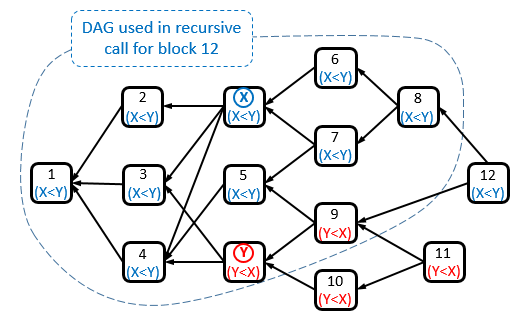
\includegraphics{figures/SPECTRE}}%
	}
\caption{An example of the voting procedure in the DAG for blocks $x$ and $y$ in SPECTRE}
\end{figure}

According to rule 4, block $x$ votes for $x \prec y$, block $y$ votes for $y
\prec x$.

According to rule 1, blocks 6, 7 and 8 vote for $x \prec y$, blocks 9, 10 and 11
vote for $y \prec x$.

According to rule 2, block 12 votes according to its past. Since not all blocks
of its past have voted, we change global view to block 12's local view, which
means block 10 and 11 are excluded.

According to rule 3, block 5 votes for $x \prec y$, since the majority of its
future vote in favor of $x$ over $y$ (blocks 7, 8 versus block 9). Note that the
current view is block 12's local view and block 11 is exculded, so we cannot
take its vote.

Also according to rule 3, blocks 1\textasciitilde4 vote for $x \prec y$.

Now all the blocks in block 12's past have voted. Block $x$ gets 10 votes. Block
$y$ gets 2 votes. Block 12 follows the majority and votes for $x \prec y$ thus.


\subsubsection*{Confirmation Time}

When a node $v$ receives a block $x$, it loops to calculate the  risk of
the block. It accepts the block when the risk is smaller than a given threshold
$\epsilon$. The confirmation time of block $x$ in node $v$ is the time
since $x$ is received by $v$ until $x$ is accpeted by $v$.

The following algorithm below calculates the  risk of block $x$ in
$G_t^v$, where $G_t^v$ is the block DAG that $v$ observes at time $t$.

\begin{codebox}
\Procname{\proc{Risk}$(G_t^v, x)$}
\li \If $time\_now < publication(x)$
\li   \Then
        \Return 1
      \End
\li $T \gets time\_now - received^v(x)$
\li $G_x \gets G_{received^v(x) + 2 \cdot d} \cup future(x, G_t^v)$
\li $g \gets \min_{x' \in \overline{ainticone}(x,G_x)} |future(x',G_x)|$
\li \Return $risk\_hidden(T,g)$
\end{codebox}

The formula $risk\_hidden(T,g)$ is defined as:

$$
risk\_hidden(T,g) := \sum_{l=0}^{\infty} \pi(l) \sum_{m=0}^{\infty} Poiss((T + 2
\cdot d) \cdot \alpha \cdot \lambda, m) \cdot \left(\frac{\alpha}{1 -
\alpha}\right)^{(g - l - m)^+},
$$

where

\begin{itemize}
	\item $d$ is the upper bound on the recent delay diameter in the network,
	\item $\alpha$ is the attacker’s relative computational power,
	\item $\lambda$ is the block creation rate,
	\item $Poiss(a, b)$ is defined as $e^{-a} \cdot \frac{a^b}{b!}$,
	\item $x^+$ is defined as $\max\{0, x\}$,
	\item and $\pi$ is the stationary distribution which we will explain below.
\end{itemize}

$risk\_hidden(T,g)$ upper bounds the probability that block $x$ is preceded by
some attacker’s block $y$ in pairwise order, where $y$ is published later than
$x$.

$\pi$ is actually a vector. Informally, it is the statistical distribution of
how much more blocks attacker nodes have created than honest nodes have created
since block $x$ is published, which is called gap in the SPECTRE paper. $\pi(l)$
is the probability that the value of gap is $l$.

The value of gap changes as time goes on, forming a random walk which induces an
ergodic Markov chain. Theorietically, it could be any integer ranging from
negative infinity to positive infinity. In the worst case, it is always
non-negative. Only when the gap is non-negative is there a risk for block $x$ to
be received less or equal votes than some attacker’s block $y$ which is
published later than $x$, so that $y$ precedes $x$ in pairwise order. This is
why in the formula of $risk\_hidden$ the index $l$, i.e. the value of gap,
starts out equal to 0 instead of negative infinity.

Since the random walk of $l$ induces an ergodic Markov chain, $l$ has a unique
stationary distribution, which is $\pi$. In order to calculate $\pi$, we need to
calculate the transition probability matrix of the random walk.

Suppose that the value of $l$ ranges from 0 to $N$, where $N$ is infinity in the
above definition. We define the transition probability matrix as an $N$ by $N$
matrix $T$. We also denote by $\delta := \alpha \cdot \lambda \cdot d$. For all
$1 \leq l < N - 1$, $T_{l-1,l} = 1 - \alpha, T_{l+1,l} = \alpha$, and for $l = N
- 1$: $T_{l-1,l} = 1 - \alpha, T_{l,l} = \alpha$. The first column of the matrix
is defined by: $T_{0,0} := (1 - \alpha) \cdot e^{-\delta}, T_{1,0} = e^{-\delta}
\cdot \alpha + e^{-\delta} \cdot \delta$, for $1 < l < N - 1$: $T_{l,0} =
e^{-\delta} \cdot \frac{\delta^l}{l!}$, and $T_{N-1,0} = 1 - e^{-\delta} \cdot
\left[\frac{\delta^0}{0!} + \frac{\delta^1}{1!} + \cdots +
\frac{\delta^{N-2}}{(N-2)!}\right]$.  $\pi$ is the eigenvector of $T$
corresponding to the eigenvalue 1, where $\pi(l) \geq 0$ and the sum of $\pi$ is
1.

In practice, $\pi(l)$ is very close to zero when $l$ is very large, so we can
just pick some $N \gg 1$ instead of infinity. Therefore, the formula of
$risk\_hidden$ becomes

$$
risk\_hidden(T,g) = \sum_{l=0}^{N} \pi(l) \sum_{m=0}^{\infty} Poiss((T + 2 \cdot
d) \cdot \alpha \cdot \lambda, m) \cdot \left(\frac{\alpha}{1-\alpha}\right)^{(g
- l - m)^+}.
$$

It is recommended to calculate $\pi$ with some well-tested Markov chain library such
as the markovchain package in R.

The sum of series with index $m$ seems to be a sum of infinite series. However,
for $m > g - l$ we have $(g - l - m)^+ = 0$ and
$\left(\frac{\alpha}{1-\alpha}\right)^{(g - l - m)^+} = 1$.

Therefore, the formula of $risk\_hidden$ can be further converted as below,
where $Poiss_{cdf}$ is the cumulative distribution function (CDF) of Poisson
distribution.

\begin{align*}
risk\_hidden(T,g)
=& \sum_{l=0}^{N}\pi(l)\sum_{m=0}^{\infty}Poiss((T+2 \cdot d) \cdot \alpha \cdot \lambda, m) \cdot (\frac{\alpha}{1-\alpha})^{(g-l-m)^+} \\
=& \sum_{l=0}^{N}\pi(l) (\sum_{m=0}^{g-l}Poiss((T+2 \cdot d) \cdot \alpha
	\cdot \lambda, m) \cdot (\frac{\alpha}{1-\alpha})^{(g-l-m)} + \\
& \sum_{m=(g-l+1)^+}^{\infty}Poiss((T+2 \cdot d) \cdot \alpha \cdot \lambda, m)) \\
=& \sum_{l=0}^{N}\pi(l) ( \sum_{m=0}^{g-l}Poiss((T+2 \cdot d) \cdot
	\alpha \cdot \lambda, m) \cdot (\frac{\alpha}{1-\alpha})^{(g-l-m)} + \\
& (1 - Poiss_{cdf} ((T+2 \cdot d) \cdot \alpha \cdot \lambda, (g-l)^+))).
\end{align*}

With the converted formula we are able to calculate $risk\_hidden$ in numerical way. Figure 5 simulates the confirmation time on different block rates, it show that SPECTRE could achieve 5 seconds confirmation time on block rates higher than 10 blocks per second and 10\% faulty percentage, which is considerably promising.

\begin{figure}[ht]
	\centerline{%
	   \resizebox{0.8\textwidth}{!}{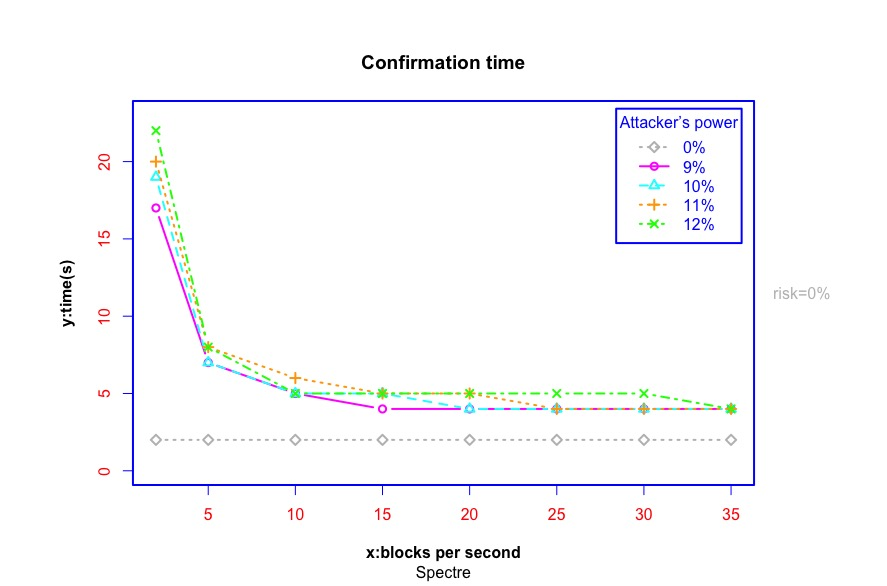
\includegraphics{figures/confirmation.jpeg}}%
	}
\caption{Confirmation Time}
\end{figure}

\subsubsection{GHOSTDAG}


Qitmeer is designed for decentralized payment network. In most scenarios , it is sufficient to provide only partial ordering or pairwise ordering for blocks in the ledger. However, sometimes it may still need to obtain a total (linear) ordering of all the blocks, especially in the event of rewarding blocks based on their ordering. 

Obtaining total ordering for a DAG ledger is not so intuitive as it is for blockchains due to a DAG ledger contains forks, which are caused by various factors, such as, network propagation delay, concurrent block creations, faulty miners. Therefore, as a supplement to the consensus protocol of Qitmeer, it uses GHOSTDAG to obtain the total ordering to reward blocks which appears earlier in the ordering.

In addition to total ordering, GHOSTDAG also provides Strong Liveness guarantee to make the consensus protocol more robust, which means both honest blocks and malicious blocks can be confirmed within a definite time, though it may take a long time to confirm malicious blocks.

Suppose that the maximal limits of network propagation delay and block creation
rate are constant. It is intuitive that if nodes behave honestly, it forms a subgraph where each block has at most a constant number of forks. We denote
this constant number as $k$. $k$ can be calculated from propagation time and
block creation rate. The subgraph is denoted as a $k$-cluster. The biggest
$k$-cluster is called a blue set. Those blocks outside the blue set are called
red set.

If we can traverse from block $x$ to block $y$ by following the parent
references within each block, then we say that there's a partial order between
$x$ and $y$, and $y$ is prior to $x$. For example in the following figure, we
can traverse from block J to A through B, so there's a partial order between A
and J, and A is prior to J. Note not all blocks have partial orders with other
blocks. For example, there are no partial orders between B, C and D.  The block set where no partial order exists is an anticone. The size of any anticone in
a $k$-cluster is at most $k$.

\begin{figure}[ht]
	\centerline{%
	   \resizebox{0.8\textwidth}{!}{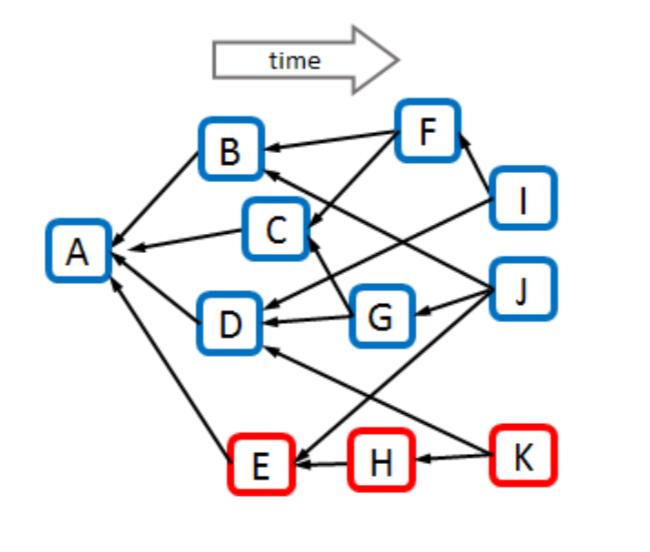
\includegraphics{figures/GHOSTDAG}}%
	}
\caption{GHOSTDAG}
\end{figure}


GHOSTDAG orders the DAG ledger in a way that favours blue blocks and penalizes
red ones. It determines the order between blue blocks according to their partial orders and some topological sor. Then, for any blue block $B$, add to the order
just before $B$ all of the red blocks in $past(B)$ that weren’t added to the
order yet; these red blocks too should be added topologically. Notice
that for any blue block $B$, the order on blocks in $past(B)$ should remain the
same if we remove from the DAG blocks in $future(B)$.

An example of the output order of the GHOSTDAG procedure on the small DAG ledger
from the figure above is: $(A,D,C,G,B,F,I,E,J,H,K)$. Nevertheless, finding the
maximum $k$-cluster is NP-hard, so GHOSTDAG is therefore of less practical use
for an ever-growing DAG ledger and may cause long confirmation times.
Therefore, we use GHOSTDAG only to implement the reward mechanism of Qitmeer, since
it should be acceptable for a miner to wait for a while to get his or her mining
reward. The confirmation time for a transaction to be accepted is still defined
in the SPECTRE way.

\subsection{Mining Algorithm}
\subsubsection{BlockDAG and Mining}
BlockDAG’s collaboration model provides much more fairness than the competition model of BlockChain on the protocol perspective. Every node gets rewards according to its contribution, re gardless of how much hash power it possess. Qitmeer favors fairness over the scalability owing to the former is more in line with true spirit of blockchain. The intention of Nakamoto Consensus is fair - every node votes with electricity; however, only a small bunch of the mining pools have the odds to participate in consensus. solo miners suffer huge opportunity cost since they have to wait for an uncertain time, quite long in most cases, to mine a block to cover their cost; thus finally it will have to turn to the mining pools. BlockDAG incorporates every miner’s block, the miners have a strong expectation of their return and then discourage to join a mining pool.


In addition, the mining algorithm is  another factor of fairness. Mining fairness refers to a certain amount of mining cost, such as electricity in POW, should derive the relatively equivalent amount of hash power. Practically, the ASIC mining rigs have much more mining efficiency than their prices.

\subsubsection{Cuckoo-Cycle-PoW}
Proof-of-Work(PoW) is used to confirm transactions and produces new blocks, and acts as the driving force in PoW based cryptocurrencies. PoW must not enable a participant to have a significant advantage over another participant. That is why Satoshi said: "Proof-of-work is essentially one-CPU-one-vote."

However, most widely used proof-of-work algorithms, such as SHA-256, Blake2b, Scrypt, are more efficient on ASIC devices when compared to CPUs and GPUs. This can lead to ASIC owners posses a much larger voting power than CPU and GPU owners, which violates the “one-CPU-one-vote” principle.

Cuckoo-Cycle-PoW, a graph-theoretic proof-of-work algorithm/ASIC-Resistant, is designed to find certain subgraphs in large pseudo-random graphs. This algorithm is ASIC resistant which  utilizes almost all parts of consumer-grade hardware in the  (GPUs, Graphic Processing Unit),

The Cuckoo Cycle POW is designed to find certain subgraphs in large pseudo-random graphs. In particular, Search for cycles of specified length L in a bipartite graph with M edges of N nodes. If a cycle is found and the hash difficulty is less than the target difficulty, the cuckoo cycle PoW is completed.




\textbf{Edge(Node) generation}

For the sake of simplicity, we define 32 edges for the bipartite graph. We call the SIPHASH function twice to create two edge endpoints(U and V), with the first input value being 2 * nonce, and the second 2 * nonce+1. The key for this function is based on a hash of a block header.

\begin{equation}
{U = SIPHASH(headerHash, 2*nonce) \mod 31}
\end{equation}
\begin{equation}
{V = SIPHASH(headerHash, 2*nonce+1) \mod 31}
\end{equation}

where,
\begin{equation}
0\leq\ {\bf nonce} \leq 31
\end{equation}it is any number between 0 and 31. Each nonce corresponds to two edge endpoints(U and V).

To throw 32 edges into a graph, randomly:

\begin{figure}[ht]
	\centerline{%
		 \resizebox{0.8\textwidth}{!}{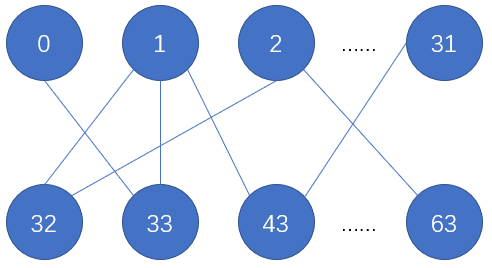
\includegraphics{figures/edge_generation}}%
	}
	\caption{Building Nodes.}
\end{figure}


\textbf{Edge Trimming}

There is a special edge in bipartite graph, which is leaf edge, and could never be part of a cycle. Leaf edge has a feature that the nodes it connects must have at least one node with the degree of the nodes being one. By eliminating leaf edge in the bipartite graph, it could greatly reduce the complexity of the graph, thus speeding up finding cycle from the bipartite graph.

\begin{figure}[ht]
	\centerline{%
		 \resizebox{0.8\textwidth}{!}{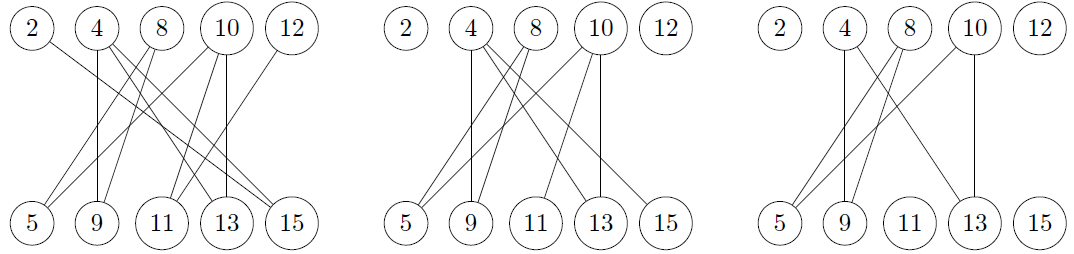
\includegraphics{figures/edge_trimming}}%
	}
	\caption{Trimming of edges which cannot be part of a cycle.}
\end{figure}

\begin{itemize}
	\item Step 1: node 0, node 3 and node 10 are one degree nodes, eliminating the edge (0,13), (6, 3) and the edge (10,9).
	\item Step 2: node 9 and node 13 are one degree nodes, eliminating the edge (8,9) and the edge (2,13).
	\item Step 3: node 8 is one degree nodes, eliminating the edge (8,11).
\end{itemize}


\textbf{Cycle detection}

After edge trimming, if a cycle of length L is found, we think we have found a solution to this problem.
we store the cycle edges in a set and put the nonce of the generated cycle in a set and
return as the result of cycle detection.


\textbf{Difficulty control}

The difficulty of finding a cycle in the graph is proportional to M/N. Here M stands for edges of the graph.
N stands for nodes of the graph. However, the difficulty of finding a cycle in the graph change is not smooth.
For crypto currencies, difficulty control must be scale in precisely controlled manner. The usual practice is
that the ratio of M/N remain fixed, such as M/N = 1/2.

Thus in the actual use, it also adds a hash difficulty control similar to Bitcoin. The digest of the cycle nonces is obtained by a hash function,
and then compared with the target difficulty.

\subsection{Rewards}
\subsubsection{Transaction Collision}
Due to asynchronous block submmission, BlockDAG protocols inevitably incorporate repeating transactions, called transaction collisons.
Miners tend to pack the transaction with higher fees to maximize their profit. This will result in high repetition rates of blocks. Repeated transactions will not contribute to the throughput, what is more, low fee transactions would wait indefinite time to get confirmed. In a fully decentralized network, nodes cannot coordinate each other to avoid collision, leaving the only option to deivse a sophiscated incentive mechanism to penalize the selfish mining behaviors.

The intuitive way to solve this challenge is to share the transaction fee, and this method will make all the miners reach a Nash equilibrium that all the miners will choose transactions randomly from their memory pools. This approach will considerably reduce transactions collision; however, users can no longer pay higher fees to boost their transaction confirmation.

Qitmeer appreciates Inclusive protocol work and adopts which states that this mechanism has some security concerns due to the fact that  it would not penalize those malicious parties who mine blocks in private. Inclusive protocol fixes this problem by only giving rewards to blocks  which are not deviating from the main chain significantly. 

\subsubsection{First Come First Serve}
The miners will encourage to submit blocks immediately upon the creation of the transaction. The transaction fee belongs to the first miner who initiated the transaction. However, this reward mechanism requires transactions has a global order, which has been offered by GHOSTDAG protocol.

Inclusive protocol states that this machanism has some security concerns because it won't penalize those malicious parites who mine blocks in private. Inclusive protocol fixes this problem by only giving rewards to blocks not deviating main chain too much. Qitmeer appreciates Inclusive protocol work and adopts it.

\section{Protocols and Interoperability}
BlockChain is the digital infrastructure for decentralized financial system, which would evolve into a complete ecosystem in the course of reaching maturity. This session analyses the typical applications available on  Qitmeer network and the protocols for interaction with Qitmeer. 

\subsection{Mining Protocol}
\subsubsection{Proof-of-work Algorithm}

The mining protocol is resistant to the centralization of mining power, which enables miner utilize almost all parts of commodity hardware (GPUs, CPUs).
Therefore, Qitmeer uses a Proof-Of-Work algorithm called Cuckoo Cycle\cite{cuckoocycle},
a memory-hard algorithm. This algorithm is designed to find certain subgraphs in large pseudo-random graphs.
An introduction of Qitmeer proof-of-work can be found here.\cite{qitmeerpow}

\subsubsection{Miner Capability}

The Qitmeer-Miner supports both solo mining and pool mining.

\subsubsection*{Solo}
If the miner  decided to mine Qitmeer without joining a pool, he would launch Solo mining mode. Solo miner connects one full node, call RPC service to mine blocks. Solo miner is recommended GPU implementation to gain better efficiency.

\subsubsection*{Pool}
Qitmeer mining pools support stratum mining protocol as most PoW mining pools do.
For example:

\emph{miner.exe -o stratum+tcp://serverIp:3177 -m YourWalletAddress.YourMachineId}

\subsection{Wallet Protocol}
\subsubsection{Overview}
   The blockchain wallet itself does not store any digital currency, and is primarily a computer program for creating digital currency transactions, tracking balances, and making it easy for users to manage addresses and private keys. Wallet software is the foundation of the whole block chain ecological development, any industry service can be realized through a block chain wallet value, block chain technology itself will reconstruct the traditional Internet business model in its own way. 
\subsection*{Openness}
   An excellent blockchain public chain project should be more inclusive and open. Therefore, in addition to its own official wallet, Qitmeer has designed all interfaces and SDK for third-party wallet development at the beginning of development. Third party wallet institutions can use these interfaces to develop a variety of wallet programs that support Qitmeer Token transactions. Including: HD wallet, SPV wallet, browser wallet to meet a variety of user needs.
\subsection*{How to create a wallet}
   The following is a simple wallet creation and transaction steps:
\begin{enumerate}
	\item  Generate seeder.
    \item  Derive private key.
    \item  Derive public key.
    \item  Derive address.
    \item  Monitor for outputs.
    \item  Create unsigned Transactions.
    \item  Sign Transactions.
    \item  Broadcast Transactions.
\end{enumerate}

   To complete the above operations, we need to rely on qitmeer's Qitmeer SDK and RPC interface.
   The Qitmeer SDK is a collection of tools that integrates various encryption, decryption, and signature functions. We can use the Qitmeer SDK to develop the following functions:

   \begin{enumerate}
     \item Generate seeder.
     \item Derive private key.
     \item Derive public key.
     \item Derive address.
     \item Create unsigned Transactions.
	 \item Sign Transactions.
   \end{enumerate}

   RPC is a http-based network interface, it’s easy to interact with qitmeer network. We can use the Qitmeer SDK to develop the following functions:

   \begin{enumerate}
    \item  Get block count from block dag or block chain.
    \item Get block data with block height.
    \item  Gettransaction data with txid.
    \item  Gets all transaction data waiting for confirmation.
    \item  Monitor for outputs.
    \item  Broadcast Txes.
   \end{enumerate}


\subsection{Cross Chain}
Qitmeer is dedicated to undertake the tokenized liquidity and host applications of global ecosystem of Islamic finance. Consequently the design goal of Qitmeer is to build up a simple and robust UTXO-based value transfer network, which prefers interoperability solutions to integrate various blockchains and applications, such as smart contract. Eventually, they will be part of Qitmeer’s ecosystem and can interact with each other.

\subsubsection{UTXO interoperability}
Currently, Qitmeer has supported P2SH script contracts and cross-chain functions through hash-locking.

\subsubsection*{Process (BTC to MEER)}

The implementation process of hash locking across the chain is:

\begin{enumerate}
\item  Alice and Bob generate their addresses on 'MEER' and 'BTC' chains respectively;

\item Alice generates her own Secret Key and Secret Key hash;

\item Alice locks her 'MEER' token into the hash lock contract in the main chain of 'MEER'. The unlock condition is that Bob holds the Secret Key or returns it to Alice after exceeding the specified time;

\item Bob checks the contract of Alice's main chain in 'MEER' and USES to generate the corresponding contract in 'BTC'. The unlock condition is that Alice holds the Secret Key or returns it to Bob after the specified time;

\item Alice USES to remove Bob's lock 'BTC' in the hash lock contract;

\item After obtaining , Bob locks Alice 'MEER' in the hash lock contract, and completes the transaction;

\end{enumerate}

\begin{figure}[hbt]
	\centerline{%
	   \resizebox{0.8\textwidth}{!}{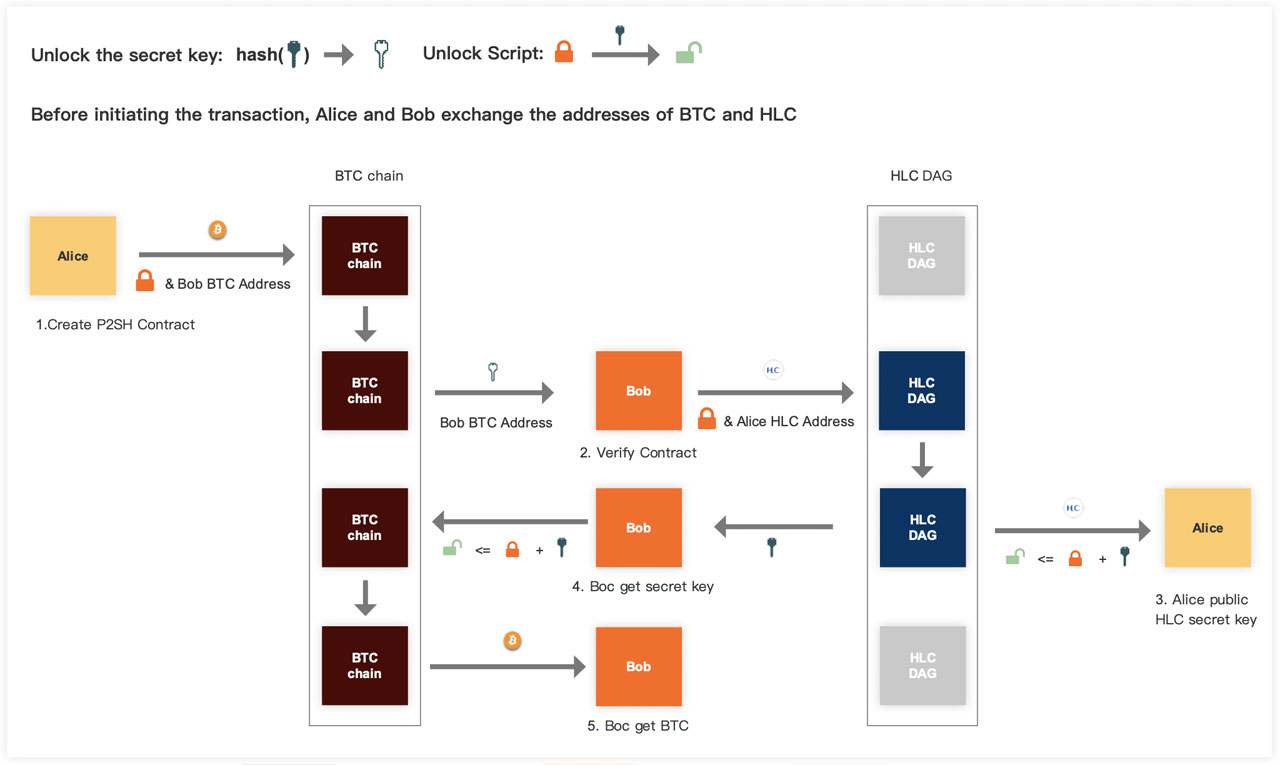
\includegraphics{figures/UTXOAtomicSwap.jpg}}%
	}
\caption{UTXO}
\end{figure}



\subsubsection{Smart Contract Interoperability}

Qitmeer completes the cross- chain transaction between the block chain assets of Qitmeer and  other account models through hash lock Smart contract.

\subsubsection*{Smart Contract Interoperability Process (ETH to MEER)}

\begin{enumerate}
\item  Alice and Bob generate their addresses on 'MEER' and 'ETH' chains respectively;

\item   Alice generates her own Secret Key and Secret Key hash;

 \item  Alice locks her 'MEER' token into the hash lock contract in the main chain of 'MEER'. The unlock condition is that Bob holds the Secret Key or returns it to Alice after exceeding the specified time;

 \item  Bob checks the contract of Alice in the main chain of 'MEER' and generates the corresponding contract on 'ETH'. The unlock condition is that Alice holds the Secret Key or returns it to Bob after exceeding the specified time.

 \item  Alice USES to call Smartcontract to remove 'ETH';

 \item  After obtaining , Bob locks Alice 'MEER' in the hash lock contract, and completes the transaction;

\end{enumerate}


\clearpage
%\appendix
%\section{Appendix}
%\begin{appendices}
%\section{append A}

%Foo bar Foo bar Foo bar Foo bar Foo bar Foo bar Foo bar Foo bar Foo bar Foo bar

%\end{appendices}

%\bibliographystyle{plainnat}
%\bibliographystyle{unsrt,acm}
\bibliographystyle{unsrt}
\bibliography{hlc_whitepaper}

\end{document}

